\section{Operación}
\label{anexo:operacion}

Tras realizar las verificaciones mencionadas en la Sec. 
\ref{anexo:verificaciones} del Manual de Usuario proceda de la siguiente
manera para la operación normal de la planta.

Normalmente, si el programa que corre en el \gls{plc} no ha sido cambiado,
usted debería ser capaz de retomar la operación de la planta mediante el 
sistema \gls{scada} (Sec. \ref{anexo:operacionSCADA} del Manual del Usuario).
En caso contrario, o para asegurarse de que el programa que corre en el
\gls{plc} es el correcto, realice los pasos que siguen a continuación.

\subsection{Carga del programa en el PLC}
\label{anexo:operacionPLC}

% \begin{enumerate}
%  \item Controlar el nivel de agua en los tanques según el anexo \ref{anexo:puestaEnMarcha}.
%  \item Controlar que las válvulas manuales estén en su correcta
%  posición según el anexo \ref{anexo:puestaEnMarcha}.
%  \item Conectar el aire a presión según el anexo \ref{anexo:puestaEnMarcha}.
%  \item Conectar la planta a la red eléctrica.
%  \item Activar en interruptor termomagnético ubicado dentro del tablero
%  eléctrico.
%  \item Conectar la planta con la computadora mediante el cable cable RS-485 
%  con adaptación a RS-232C. Puede ser necesario utilizar un adaptador
%  RS-232C/USB.
%  \item Abrir el programa del \gls{plc} denominado {\color{red}(nombre del programa)} 
%  con el Software Twido Soft. Este programa se encuentra en el DVD adjunto al
%  informe.
%  \item Conectarse al \gls{plc} como se indica en la imagen \ref{img:twidosoft}.
%  \item Cargar el programa en el \gls{plc}, imagen \ref{img:twidosoftcargar}.
%  \item Poner a correr el programa, imagen\ref{img:twidosoftrun}.
%  \item Desconectarse del \gls{plc}, imagen \ref{img:twidosoftdesc}.
% \end{enumerate}
Usted puede leer el programa que se encuentra en la memoria del \gls{plc}, o
bien escribir en ella un nuevo programa.
Para ambas tareas es necesario que el \gls{plc} se encuentre encendido y
conectado a la computadora que lo programará.
Deberá entonces:

\begin{table}[H]
\centering
\renewcommand*{\arraystretch}{0.01}
\begin{tabular}{*{2}{m{0.44\textwidth}}}
\hline
    Energizar la planta accionando el interruptor
termomagnético ubicado dentro del tablero eléctrico.
    &\begin{center}
      %\rule{0.4\textwidth}{0.3\textwidth}
      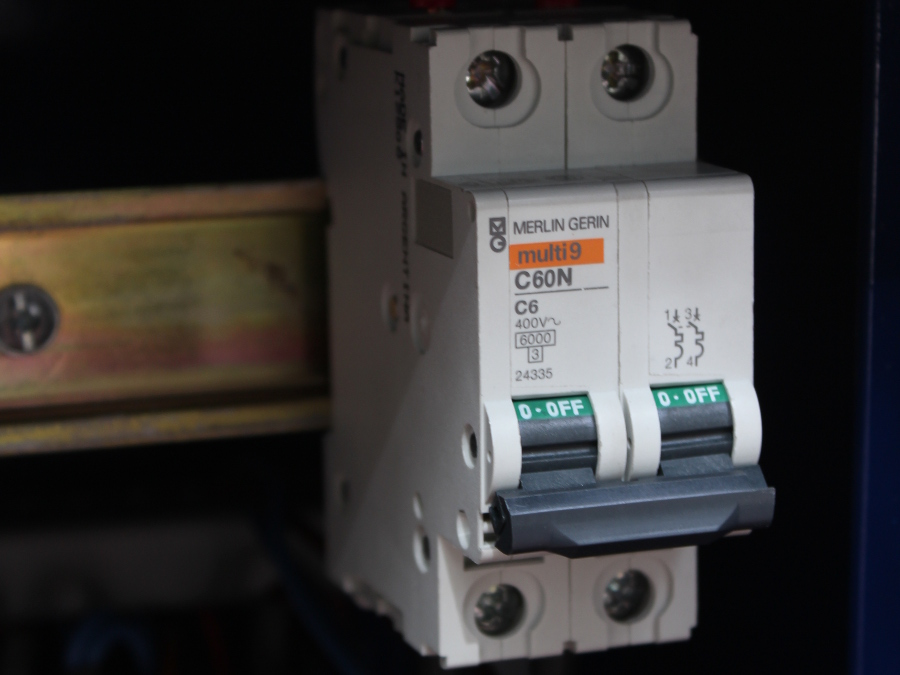
\includegraphics[width=0.4\textwidth]
	{Anexos/images/disyuntor.JPG}
    \end{center}\\
\hline
    Conectar la planta con la computadora supervisora, mediante el cable cable
\verb|RS-485|  con adaptación a \verb|RS-232C|. Puede ser necesario utilizar un
adaptador \verb|RS-232C/USB|.
    &\begin{center}
      %\rule{0.4\textwidth}{0.3\textwidth}
      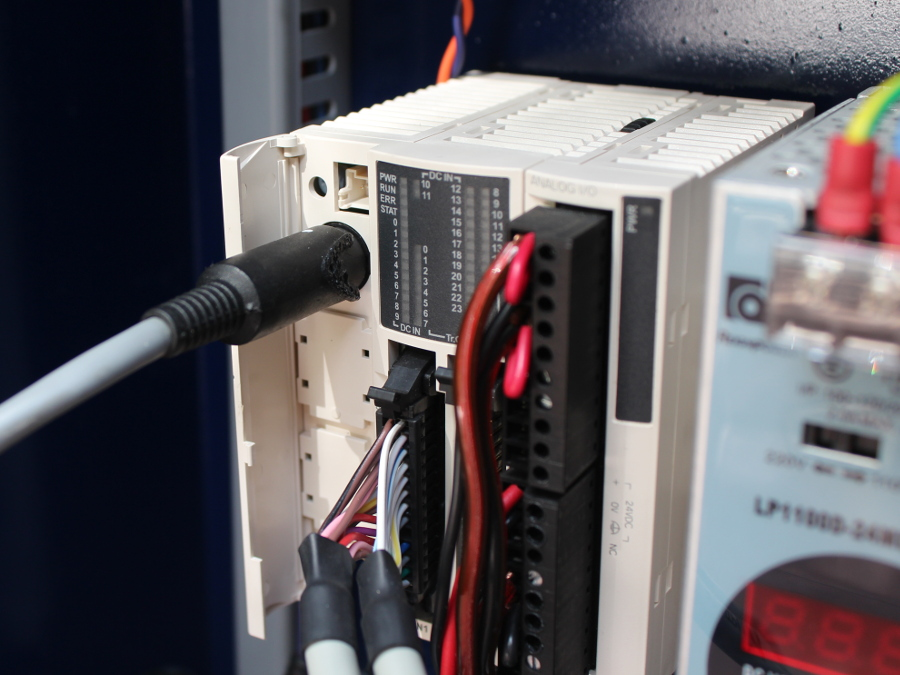
\includegraphics[width=0.4\textwidth]
	{Anexos/images/ComunicacionRs485.JPG}
    \end{center}\\
\hline
\end{tabular}
\end{table}

Se aconseja escribir y ejecutar en el \gls{plc} el programa que se encuentra en
el DVD adjunto, denominado \texttt{ABC\_plc\_1.twd}. Así, la planta
estará en un estado a partir del cual se puede operar con el sistema
\gls{scada} propuesto.

Este programa se debe abrir con el Software Twido Soft y luego proceder de la 
manera que se indica a continuación:

\begin{table}[H]
\centering
\renewcommand*{\arraystretch}{0.01}
\begin{tabular}{*{2}{m{0.45\textwidth}}}
\hline
    En la pantalla principal de TwidoSoft seleccione 
Autómata/Conectar para poder conectarse al \gls{plc}.
    &\begin{center}
      %\rule{0.4\textwidth}{0.3\textwidth}
      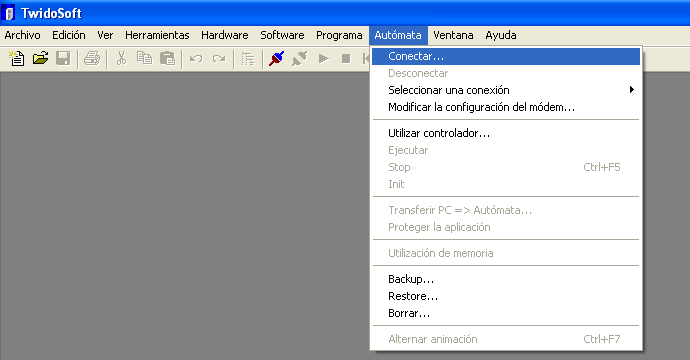
\includegraphics[width=0.4\textwidth]
	{Anexos/images/twidosoft.PNG}
    \end{center}\\
\hline
    Al conectarse el software solicitará en qué sentido debe
realizarse la transferencia de datos.
Cargar el programa desde la computadora al \gls{plc}.
    &\begin{center}
      %\rule{0.4\textwidth}{0.3\textwidth}
      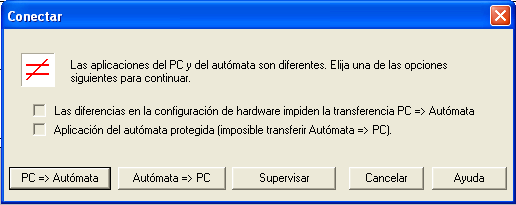
\includegraphics[width=0.4\textwidth]
	{Anexos/images/twidosoftcargar.PNG}
    \end{center}\\
\hline
    Ejecutar el programa, haciendo click el icono \emph{Run}.
    &\begin{center}
      %\rule{0.4\textwidth}{0.3\textwidth}
      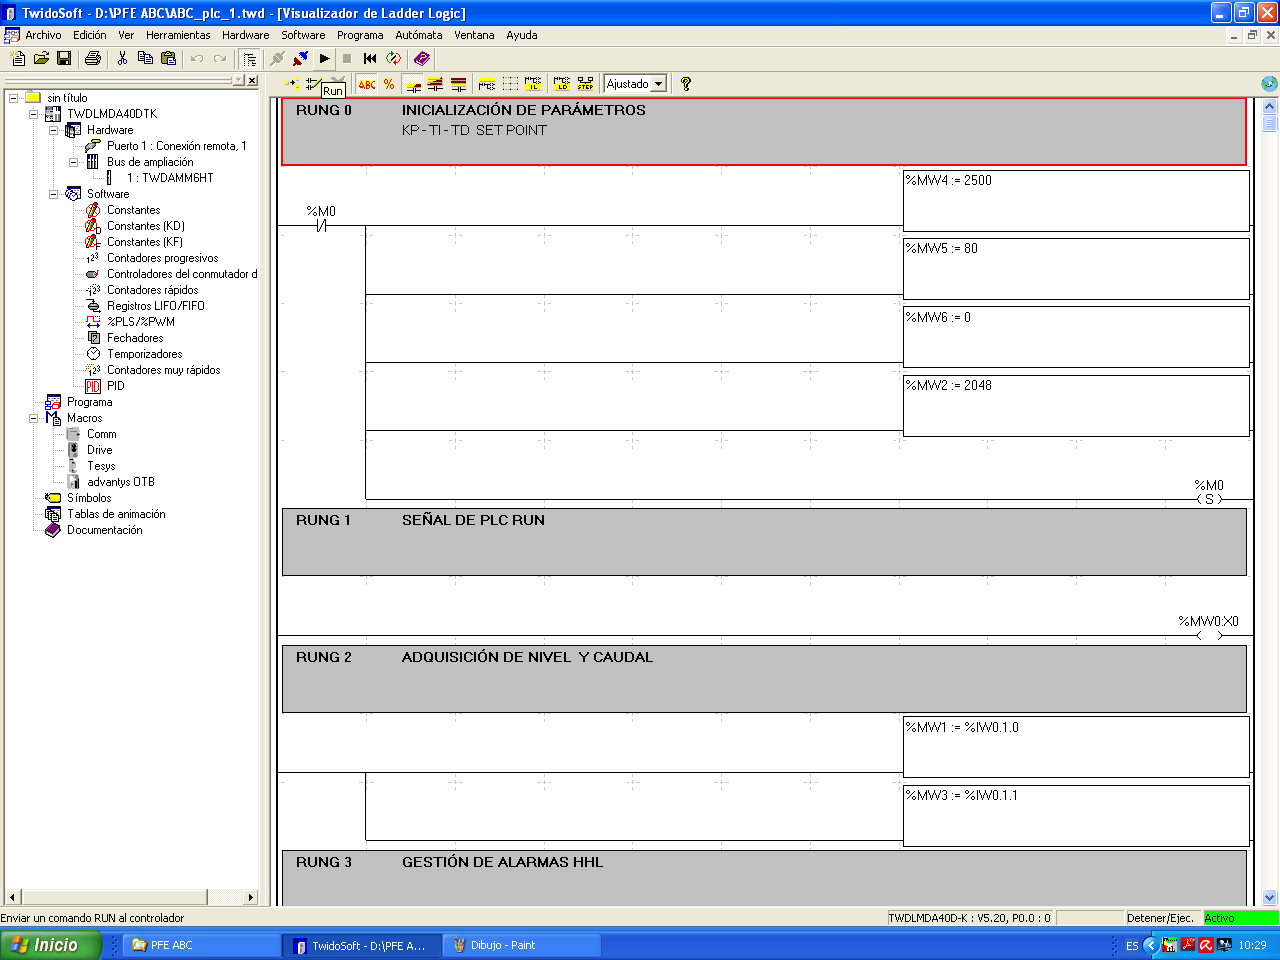
\includegraphics[width=0.4\textwidth]
	{Anexos/images/twidosoftrun.PNG}
    \end{center}\\
\hline
  Finalmente puede desconectarse del \gls{plc}
  &\begin{center}
    %\rule{0.4\textwidth}{0.3\textwidth}
    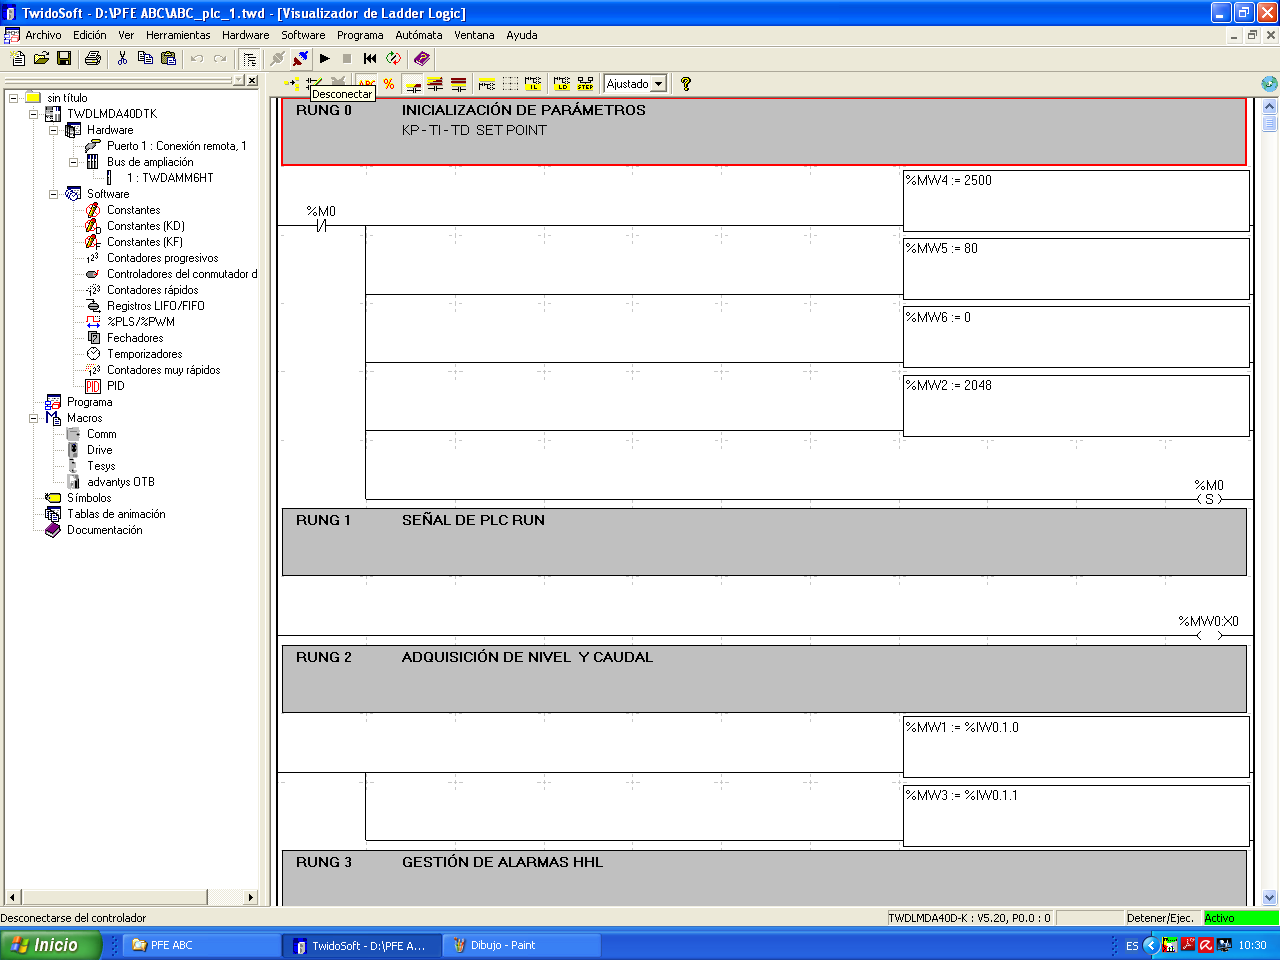
\includegraphics[width=0.4\textwidth]
      {Anexos/images/twidosoftdesc.PNG}
  \end{center}\\
\hline
\end{tabular}
\end{table}

\newpage
\subsection{SCADA}
\label{anexo:operacionSCADA}

\begin{lattention}
 Recuerde siempre realizar las verificaciones descriptas en la Sección 
\ref{anexo:verificaciones} del Manual del Usuario antes de continuar con la
operación de la planta.
\end{lattention}

\subsubsection{Restore Project}
El primer paso para utilizar el sistema \gls{scada} es recuperar el 
proyecto para AFCON P-CIM del DVD adjunto. Siga las siguientes instrucciones 
para completar esta tarea:
\begin{table}[H]
\small
\centering
\renewcommand*{\arraystretch}{0.3}
\begin{tabular}{*{2}{m{0.435\textwidth}}}
\hline
  Elija Setup de P-CIM del grupo de aplicaciones que se encuentran la carpeta 
  AFCON P-CIM[7.70SP4]. 
  &\begin{center}
    %\rule{0.4\textwidth}{0.3\textwidth}
    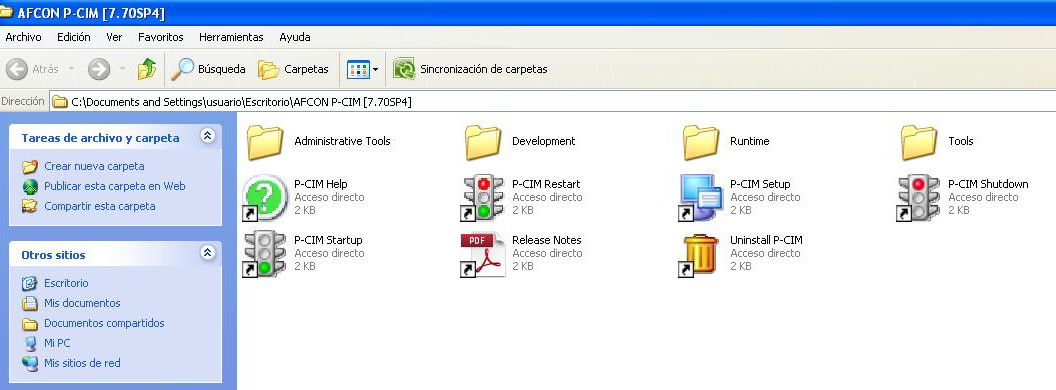
\includegraphics[width=0.4\textwidth]
	{Cap5-SCADA/images/Dibujo1.JPG}
  \end{center}\\
\hline
  De la ventana de Setup de P-CIM seleccione Restore Project.
  Se desplegará la ventana de diálogo de instalación para restaurar el proyecto.
  &\begin{center}
    %\rule{0.4\textwidth}{0.3\textwidth}
    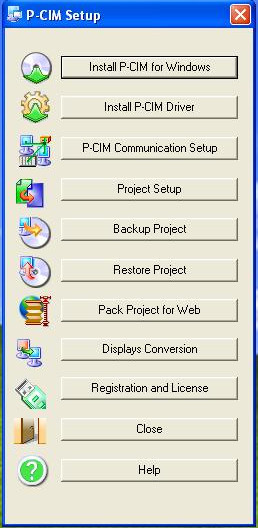
\includegraphics[height=0.3\textwidth]
	{Cap5-SCADA/images/PcimSetup.jpeg}
  \end{center}\\
\hline
  De la ventana de Restore Project oprima Browse para seleccionar la carpeta 
  PFE\_ ABC del DVD adjunto. Luego, se pedirá autorización para continuar con 
  la restauración. Finalmente, oprima Yes para hacerlo como proyecto por 
  Default.
  &\begin{center}
    %\rule{0.4\textwidth}{0.3\textwidth}
    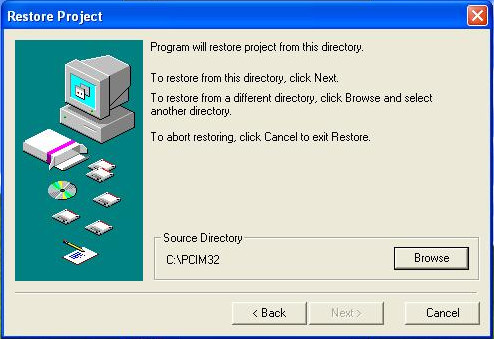
\includegraphics[width=0.4\textwidth]
	{Anexos/images/restoreProject.JPG}
  \end{center}\\
\hline
\end{tabular}
%\caption{Instalación del Driver Modbus}
%\label{tab:installModbus}
\end{table}

\subsubsection{Verificar la Comunicación}
A continuación se debe verificar que la comunicación con el \gls{plc}
se encuentra bien configurada y que el sistema \gls{scada} es capaz de
intercambiar información con el controlador.
Proceda como se describe a continuación:
\begin{table}[!ht]
\centering
\renewcommand*{\arraystretch}{0.01}
\begin{tabular}{*{2}{m{0.45\textwidth}}}
\hline
  Seleccione de la  ventana de P-CIM Setup  el botón P-CIM Communication Setup. 
  Luego, desde la ventana de diálogo ``Project Communication Setup'' 
  marque la línea correspondiente en el cuadro de Assigned ports y 
  elija  Properties.
    &\begin{center}
      %\rule{0.4\textwidth}{0.3\textwidth}
       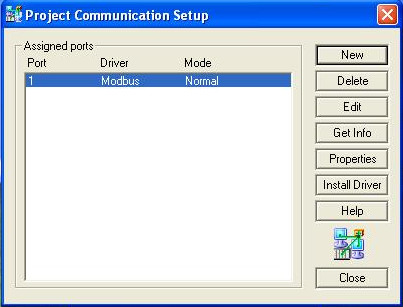
\includegraphics[width=0.4\textwidth]
	{Cap5-SCADA/images/commSetup.jpeg}
    \end{center}\\
\hline
   Se despliega la ventana P-CIM Configurator for MODBUS Driver. Verifique 
   que Network Type sea RS232. Presione el botón Transport Parameter el cual 
   despliega una nueva ventana
  &\begin{center}
    %\rule{0.4\textwidth}{0.3\textwidth}
    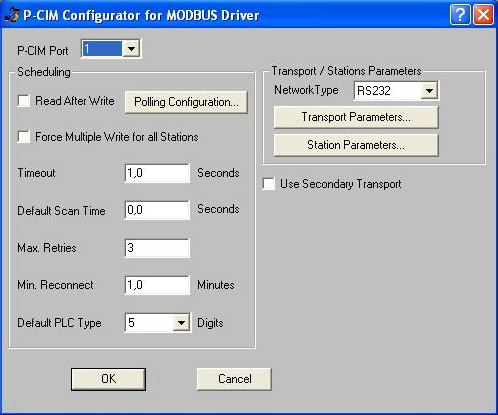
\includegraphics[width=0.4\textwidth]
      {Cap5-SCADA/images/modbusDriver.jpeg}
  \end{center}\\
\hline 
   El valor de COM Port debe ser el mismo que aparece en el Administrador de 
   Dispositivos de Windows correspondiente al puerto serie de 
   comunicaciones con el \gls{plc}. Baud Rate:19200. 
  &\begin{center}
    %\rule{0.4\textwidth}{0.3\textwidth}
        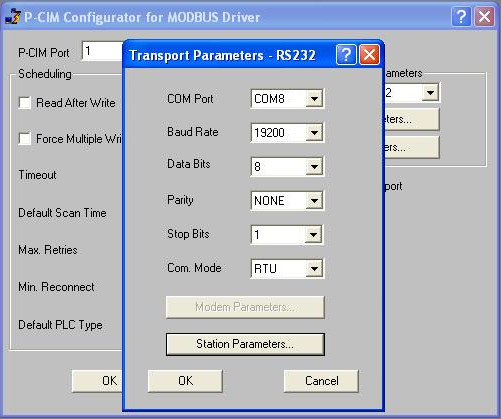
\includegraphics[width=0.4\textwidth]
      {Cap5-SCADA/images/modbusDriver2.jpeg}
  \end{center}\\
\hline
\end{tabular}
%\caption{Propiedades del Driver Modbus}
%\label{tab:PropModbus}
\end{table}


\newpage
\subsubsection{Iniciar P-CIM}
Finalmente, para controlar el sistema desde el \gls{scada} P-CIM de AFCON,
es necesario iniciar P-CIM y verificar que el driver de Modbus se haya cargado 
correctamente, permitiendo la comunicación con el \gls{scada}:
\begin{table}[!ht]
\centering
\renewcommand*{\arraystretch}{0.01}
\begin{tabular}{*{2}{m{0.45\textwidth}}}
\hline
  Active P-CIM utilizando el Startup de P-CIM del grupo de aplicaciones de la 
carpeta AFCON P-CIM.
  &\begin{center}
    %\rule{0.4\textwidth}{0.3\textwidth}
    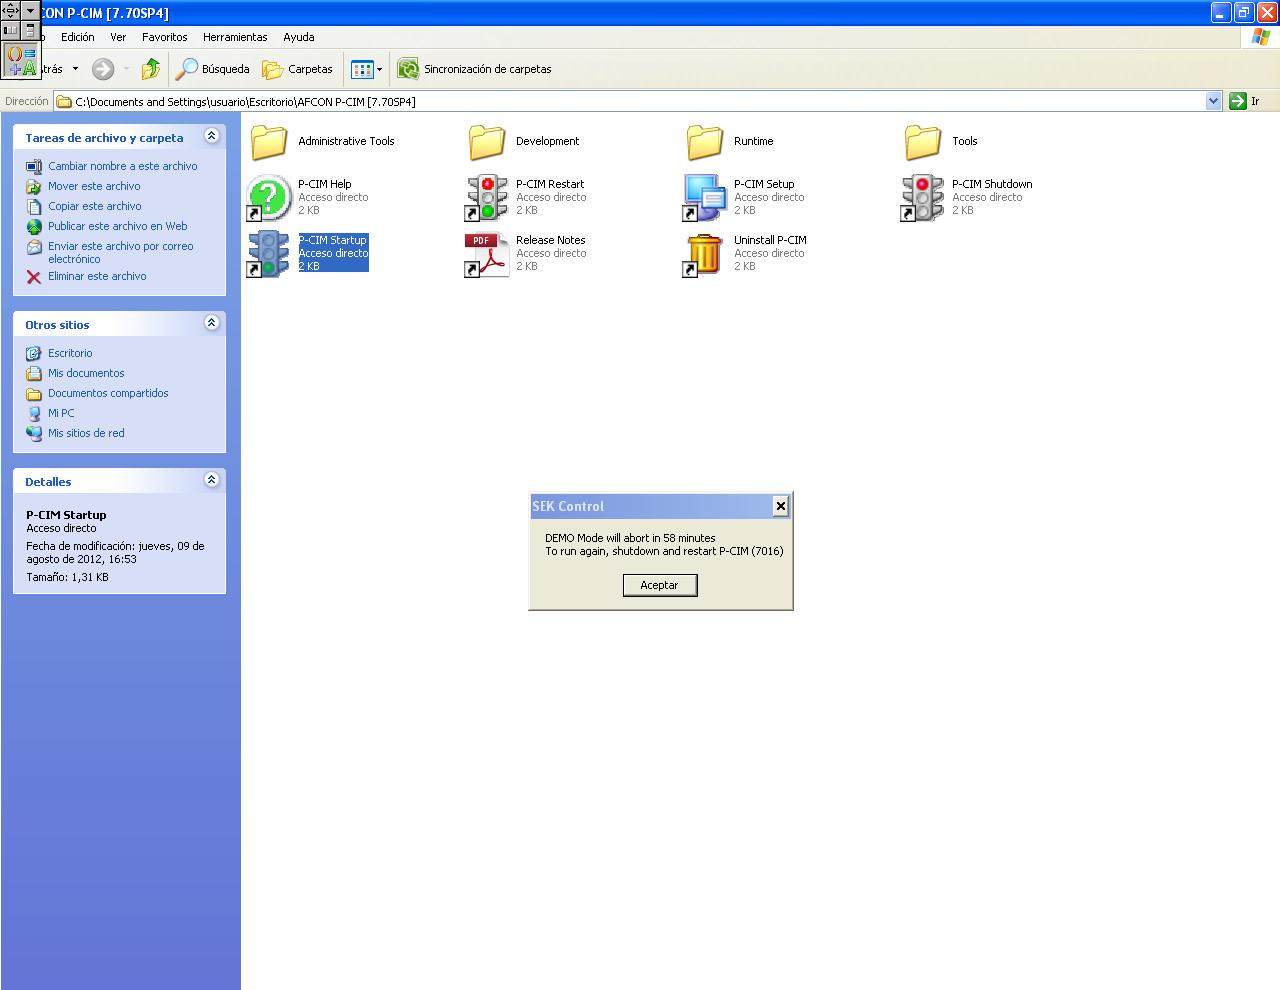
\includegraphics[width=0.4\textwidth]
      {Cap5-SCADA/images/startUp.jpeg}
  \end{center}\\
 \hline
   Verifique que en la ventana Alarm Summary muestre el mensaje “MODBUS
  Driver successfully loaded” indicando que el driver halló la tabla de 
  comunicación y fue exitosamente cargado.
  &\begin{center}
    %\rule{0.4\textwidth}{0.3\textwidth}
    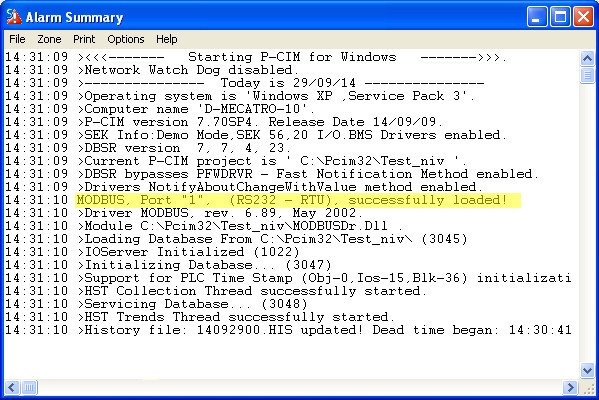
\includegraphics[width=0.4\textwidth]
      {Cap5-SCADA/images/alarm.jpeg}
  \end{center}\\
 \hline
\end{tabular}
\end{table}

\begin{lattention}
En el caso de que no se haya logrado cargar el driver Modbus refiérase a la 
Tab. \ref{tab:PropModbus} de la Sec. \ref{subsubsec:InforDriver} del Informe
de Proyecto Final.
\end{lattention}

\subsubsection{Operators Workspace}

Automáticamente tras iniciar P-CIM como se muestra en la sección anterior, se 
abrirá la aplicación Operator Workspace ejecutando el entorno gráfico del 
sistema \gls{scada}.

A través de esta interfaz es posible manejar la planta.
Pueden diferenciarse los siguientes bloques principales
(ver Fig. \ref{fig:hmiscada2}).

\begin{figure}[!ht]
	\centering
	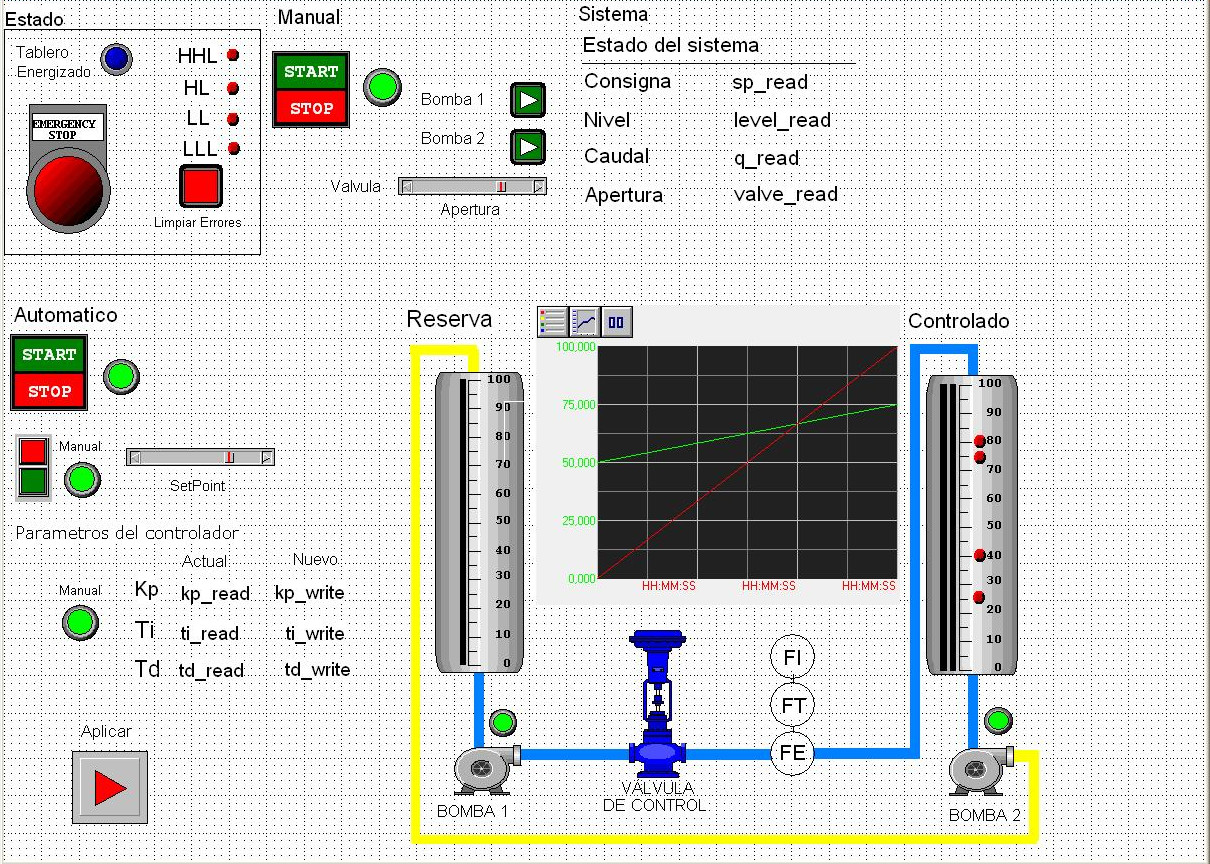
\includegraphics[width=0.8\textwidth]
	{Cap5-SCADA/images/hmiScada.jpeg}
	\caption[]{Interfaz gráfica del sistema SCADA}
	\label{fig:hmiscada2}
  \end{figure}
  
\begin{enumerate}
\item \textbf{Parada de Emergencia:} mediante este botón se detiene totalmente
la planta, y solo volverá a responder si se presiona \textbf{Rehabilitar
Sistema}.
 \item \textbf{Control Automático:} desde estos controles se activa o detiene
la planta cuando el controlador automático está activo.
 \item \textbf{Control Manual:} este modo debe ser usado solamente como un
medio para
sacar a la planta de un estado de emergencia tras  haberse declarado una alarma
por HHL o LLL.
Aquí podrá encender las electrobombas individualmente y controlar la apertura
de la válvula.
 \item \textbf{Ganancias del Controlador:} en esta sección usted puede enviar al
\gls{plc} de la planta las constantes del controlador $K_p$, $T_i$ y $T_d$. 
Puede seleccionar los valores por Default o Manual. Pulse Aplicar para que los
cambios sean efectivos.
 \item \textbf{Consigna de Nivel:} en esta sección usted puede enviar al
\gls{plc} de la planta la consigna/setpoint de nivel del tanque controlado. 
Puede seleccionar el valor por Default ($50\%$) o Manual. Pulse Aplicar para
que
los cambios sean efectivos.
 \item \textbf{Sistema:} en este apartado se puede ver el estado del actual del
sistema. Es decir, se muestran los valores de consigna de nivel, nivel
actual, caudal y apertura de la válvula. También se señalan el estado del 
\gls{plc} y si el sistema se encuentra funcionando en estado normal.
\item \textbf{Elementos Gráficos}: en ellos se pueden observar los valores
actuales e
históricos de nivel de ambos tanques. También se señalan las alarmas de nivel y
sus valores.
\end{enumerate}
